\documentclass[11pt]{article}
\usepackage[letterpaper,landscape,margin=0.6in]{geometry}
\usepackage{booktabs,graphicx,amsmath}
\setlength{\parindent}{0pt}
\setlength{\parskip}{5pt}
\begin{document}
\begin{center}\Large\textbf{Individual CCEI coefficients and relative distance to group choices}\end{center}
\small
Outcome: normalized distance of the more rational member to the group, $\widehat I_{\mathrm{more},g}$.
Both members' continuous CCEIs enter together, with category-specific slopes; no more/less-rational indicator enters.
\[
\widehat I_{\mathrm{more},g}=\alpha_c+\beta_{\max,c}\mathrm{CCEI}_{\max}
+\beta_{\min,c}\mathrm{CCEI}_{\min}+Z_g'\gamma+\lambda_{\mathrm{class}}+\varepsilon_g.
\]
\begin{center}\begin{minipage}{0.48\textwidth}\centering
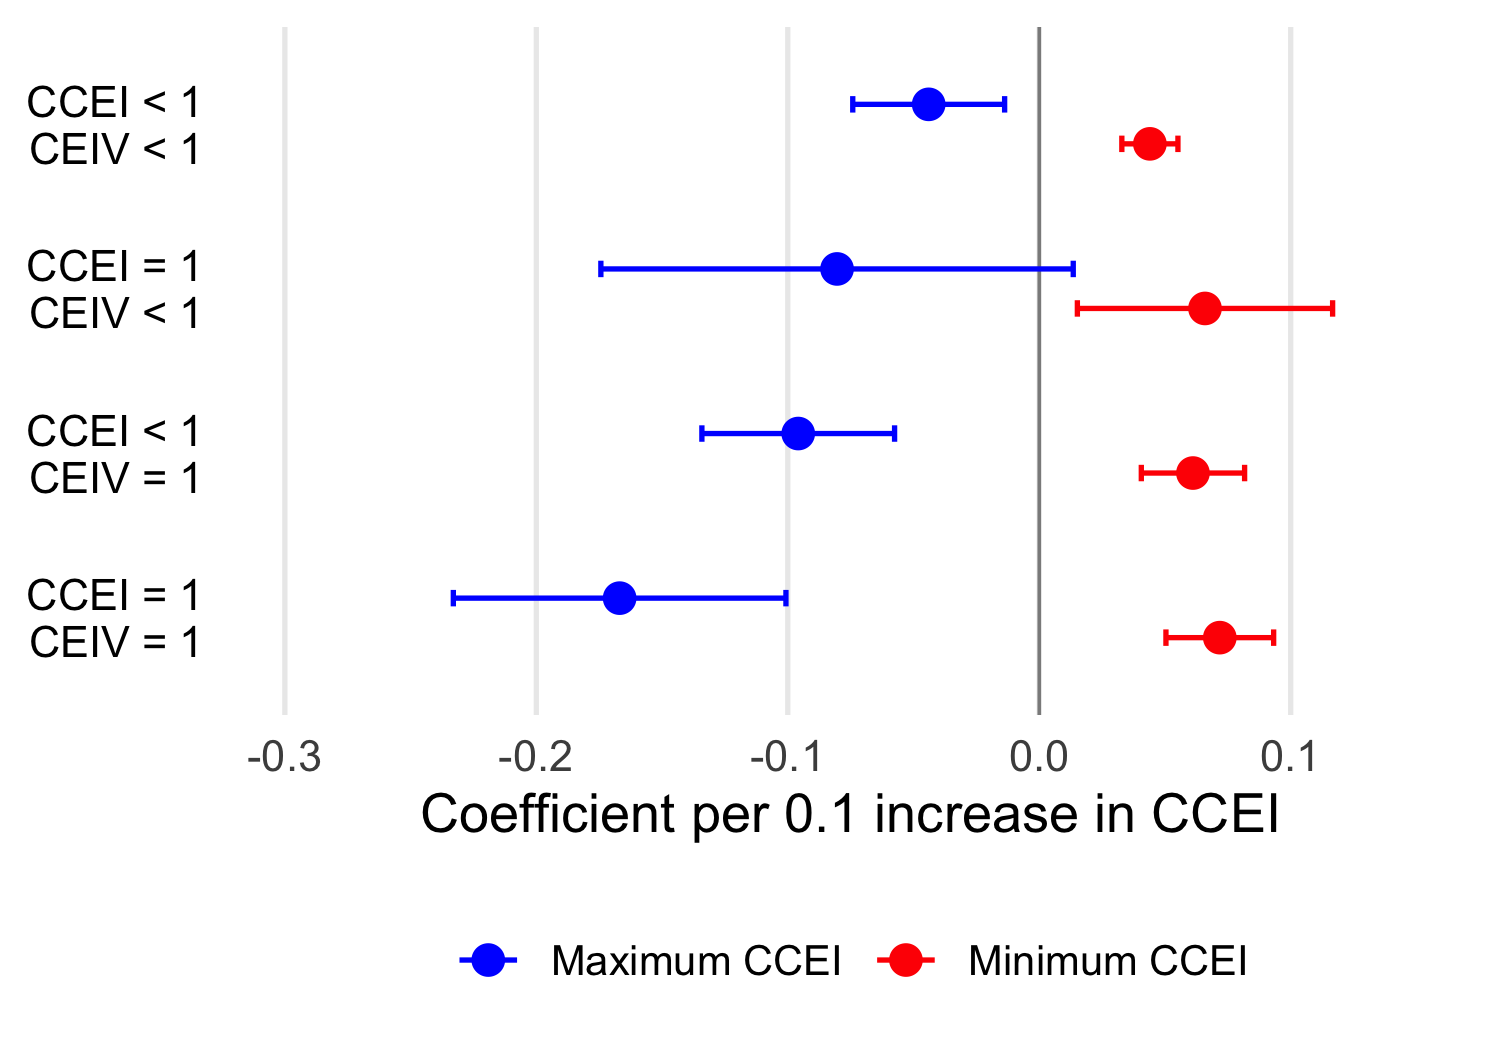
\includegraphics[width=\linewidth]{unadjusted_coefficients.png}\\
\textbf{(a) Both CCEIs and category interactions only}
\end{minipage}\hfill\begin{minipage}{0.48\textwidth}\centering
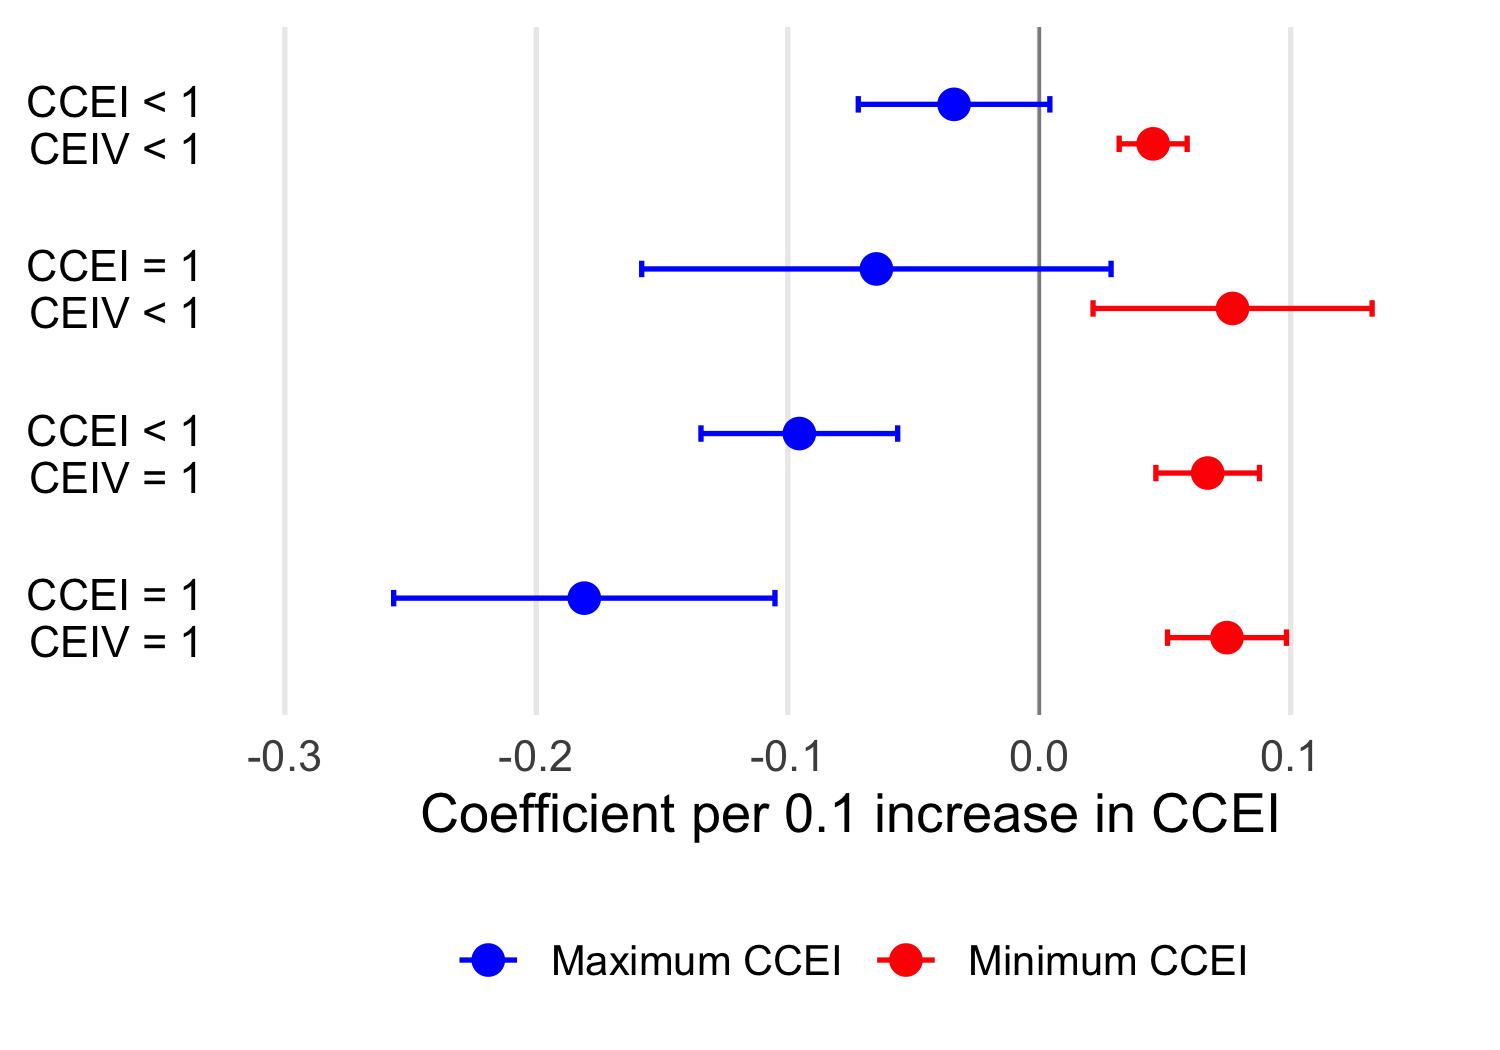
\includegraphics[width=\linewidth]{controlled_coefficients.png}\\
\textbf{(b) Other characteristics and class fixed effects}
\end{minipage}\end{center}
\begin{center}\small\begin{tabular}{lrrrrr}\toprule
& \multicolumn{2}{c}{CCEI-only specification} & \multicolumn{2}{c}{With other controls} & Pair-waves\\
Group outcomes & Maximum CCEI & Minimum CCEI & Maximum CCEI & Minimum CCEI &\\\midrule
CCEI$<1$, CEIV$<1$ & -0.044 (0.015) & 0.044 (0.006) & -0.034 (0.019) & 0.045 (0.007) & 378\\
CCEI$=1$, CEIV$<1$ & -0.080 (0.047) & 0.066 (0.025) & -0.065 (0.047) & 0.077 (0.028) & 100\\
CCEI$<1$, CEIV$=1$ & -0.096 (0.019) & 0.061 (0.010) & -0.095 (0.020) & 0.067 (0.010) & 268\\
CCEI$=1$, CEIV$=1$ & -0.167 (0.033) & 0.072 (0.011) & -0.181 (0.038) & 0.075 (0.012) & 355\\
\bottomrule\end{tabular}\end{center}
\textbf{Interpretation.} Increasing maximum CCEI predicts a smaller distance for the more rational member.
Increasing minimum CCEI predicts a larger distance for that member, hence a smaller distance for the less rational member.
Because the two distances sum to one, an identically specified regression for the less rational member has opposite
coefficients and identical standard errors. These signs describe relative alignment, not changes in absolute distance.

\footnotesize
\textit{Notes:} Table and chart coefficients are rescaled to a 0.1 increase in individual CCEI; multiply by ten for
the equation's one-unit coefficients. Parentheses contain class-clustered standard errors; bars are 95\% intervals.
Both specifications fit all 1,101 untied pair-waves with observed distances, pooling both waves, with 64 class clusters.
Controls are the Figure 6 student/personality and friendship/network controls, plus class effects, sharing control
coefficients across categories. Individual choice-share and RA controls are excluded; no wave fixed effect enters.
Near-one CCEIs have limited room to increase, so the coefficient scaling is not a feasible 0.1 change for every observation.
Categories are defined by group outcomes; coefficients are descriptive conditional associations.
\clearpage
\begin{center}\Large\textbf{Are category differences driven by different individual CCEI levels?}\end{center}
\small
Evaluate each category's fitted distance at the same two individual CCEIs. The reference values are the pooled means
among the same 1,101 included pair-waves:
$\mathrm{CCEI}_{\max}=0.967$ and $\mathrm{CCEI}_{\min}=0.834$.
The CCEI-only specification changes just these two levels. The controlled specification also averages other
characteristics and class effects over their pooled distribution. Slopes remain category-specific.

\begin{center}\begin{tabular}{lrrrrr}\toprule
& \multicolumn{2}{c}{Observed individual CCEI means} & \multicolumn{3}{c}{More rational member's distance}\\
Group outcomes & Maximum & Minimum & Raw mean & Common CCEIs & Common CCEIs + controls\\\midrule
CCEI$<1$, CEIV$<1$ & 0.955 & 0.813 & 0.431 & 0.435 & 0.435\\
CCEI$=1$, CEIV$<1$ & 0.972 & 0.880 & 0.411 & 0.385 & 0.382\\
CCEI$<1$, CEIV$=1$ & 0.960 & 0.815 & 0.360 & 0.364 & 0.365\\
CCEI$=1$, CEIV$=1$ & 0.985 & 0.859 & 0.261 & 0.273 & 0.275\\
\bottomrule\end{tabular}\end{center}
\textbf{Within CEIV$=1$: both indices equal one minus CEIV-only.}
\begin{center}\begin{tabular}{lrrr}\toprule
Comparison & Distance difference & 95\% interval & $p$\\\midrule
Raw means & -0.098 & [-0.151, -0.046] & $<0.001$\\
Common individual CCEIs & -0.092 & [-0.141, -0.042] & $<0.001$\\
Common CCEIs and other characteristics & -0.089 & [-0.143, -0.035] & 0.002\\
\bottomrule\end{tabular}\end{center}
\textbf{Finding.} The distance contrast changes from -0.098 to -0.092 when individual CCEIs are set to common levels. Most of the observed gap remains in this linear specification; differences in the distribution of members' CCEIs account for little of it. This is a model-based comparison, not a causal decomposition.

\textbf{Slope comparison.} Within CEIV$=1$, the maximum-CCEI slope is more negative when group CCEI also equals one (difference -0.086 per 0.1, $p=0.039$). The minimum-CCEI slope difference is small and imprecise ($p=0.582$).

\footnotesize
\textit{Notes:} Roles are defined separately in each wave; individual CCEI ties within $10^{-9}$ are excluded, as in
the preceding distance comparison. Four additional untied pair-waves have undefined distances. CCEI/CEIV values at
least $1-10^{-9}$ count as one. The common CCEI values are within observed joint support in each category. Predicted
distances for the less rational member are one minus those shown. Class-clustered uncertainty treats the chosen
reference CCEI values as fixed; no uncertainty is added for estimating their pooled means. The linear model allows
category-specific intercepts and CCEI slopes, and common coefficients for additional controls. These are comparisons
of groups defined by outcomes, with related revealed-preference measures computed from the same choice data;
they do not identify aggregation weights or a communication mechanism. Tests are exploratory and unadjusted for
multiple comparisons.
\end{document}
